\section{Experiments}
In 2004, there are totally 114 projects contain 1628 subproject in different locations. 
\subsection{Software packages}
Our method is based on the R package rpart \cite{cart}. Rpart support user defined split function, therefore, we can use the split criterion function \ref{eq:5}. To improve the efficiency of the r program, we use rcpp and call C++ functions inside the split and evaluation function for each node in the tree. To further improve the c++ functions, we use openmp inside the C++ functions. To avoid the extreme cases, such as only treated or untreated data in the internal nodes, we would not split under in such condition. We use the randomForest \cite{rf} R package to build the forest.

\subsection{TOT Results}
\begin{itemize}
\item observation: calculation of $/alpha$ for pruning is computationally expensive but can be parallelized. This can be done for all methods. Discuss speed up for one of the methods.
\item Resulting average treatment effect obtained from leaf node. In order to have a reasonable estimate, there is a trade off in being specific (have a refined tree with little variation but fewer units per leaf node) or being more general and have more diverse units in a leaf node but a have more values to support an estimate for an average value
\item TOT allows us to compute average treatment effect for each unit $i$
\item TOT allows us to rank covariates according to the order of variables in the tree
\item TOT allows us to find similar projects to compare based on sets of units in each leaf
\item Can not measure how representative the tree, unclear how to measure confidence in judgement etc
\item discuss the actual outcome for a single example project that serves as an illustrating example all along the other methods (may be a particular good project)
\end{itemize}

\subsection{CT Results}
\begin{itemize}
\item Resulting average treatment effect obtained from leaf node. In order to have a reasonable estimate, one needs at least one treated and one untreated unit per leaf. In order to ensure this, one can configure the splitting rule accordingly, however this may come for the price that units remain in the same set that are not very similar.
\item CT allows us to compute average treatment effect for each unit $i$ if at least one treated, untreated unit is present
\item CT allows us to rank covariates according to the order of variables in the tree
\item CT allows us to find similar projects to compare based on sets of units in each leaf
\item Can not measure how representative the tree, unclear how to measure confidence in judgement etc
\item discuss the actual outcome for a single example project that serves as an illustrating example all along the other methods (may be a particular good project)
\end{itemize}

\subsection{Random Forest Results}
\begin{itemize}
\item Resulting average treatment effect obtained from averaging the outcomes of all TOT trees in the forest. 
\item RF allows us to compute average treatment effect for each unit $i$
\item RF allows us to rank covariates according to the order of variables in the tree and quantify this in terms of quantiles (percentage of trees that use covariate among its top k covariates or alike)
\item RF allows us to find similar projects to compare based on sets of units in each leaf (
\item Can not measure how representative the tree, unclear how to measure confidence in judgement etc
\item discuss the actual outcome for a single example project that serves as an illustrating example all along the other methods (may be a particular good project)
\end{itemize}

\subsection{Comparison}


\begin{itemize}
\item variable importance, important variables should be in the top levels of the tree, important to the causal effects
\item regression variability, interval, in a forest, how stable the effect of  a project is, if the variance is small, we can trust the result
\item validate the result, one of the challenges is we do not have golden truth for the projects, we have partial result from world bank IEG which is for the assessment of the implement of the overall projects, as each projects usually have more than two sub projects on different locations, the estimation is coarse. Another source of result is from the economist result,
based on these two evaluation, we can validate our work to some extent. 

\item About $83\%$ projects in 2004 have more than 1 locations, the IEG outcomes take all of the them as a whole, in our random forest, we have causal results for sub projects, hence, one project may have both good and bad causal effects.

\item quantile for each project location, variability of the causal effects, uncertainty of the result, $8\%$ data have all causal effects have same effect, either positive or negative result, $90\%$ have either positive or negative result from quantile $25\%$ to $75\%$
 
\end{itemize}



\begin{table*}[t]
	\begin{center}
		\begin{tabular}{l | c | c | c | c}
		\hline
			WB region 						& CT 			& TOT 			& RF 			& ECON \\ \hline
			AFRICA 							& -0.0034007384 	& -0.002259834  	& -0.002070222	& -0.037396489 \\ 
			EAST ASIA AND PACIFIC 			& -0.0004073951 	& -0.002602419	& -0.002338640 	& -0.054120740 \\ 
			EUROPE AND CENTRAL ASIA 		&-0.0077536156 	& 0.026434682		& 0.027010477 	& 0.030465111 	\\ 
			LATIN AMERICA AND CARIBBEAN		& 0.0089683258	& 0.014169258		& 0.010182891 	& -0.013437384 \\ 
			MIDDLE EAST AND NORTH AFRICA 	& -0.0025123259 	& -0.017290754	&-0.015723577 	& -0.008182447 \\ 
			SOUTH ASIA 						&-0.0096351385	& -0.010894742	& -0.010095676 	& -0.081190785 \\ \hline
		\end{tabular}
		\caption{causal effect by regions}\label{table:resbyregion}
	\end{center}
	
\end{table*}



\begin{figure}
	\subfloat[good projects rank]{  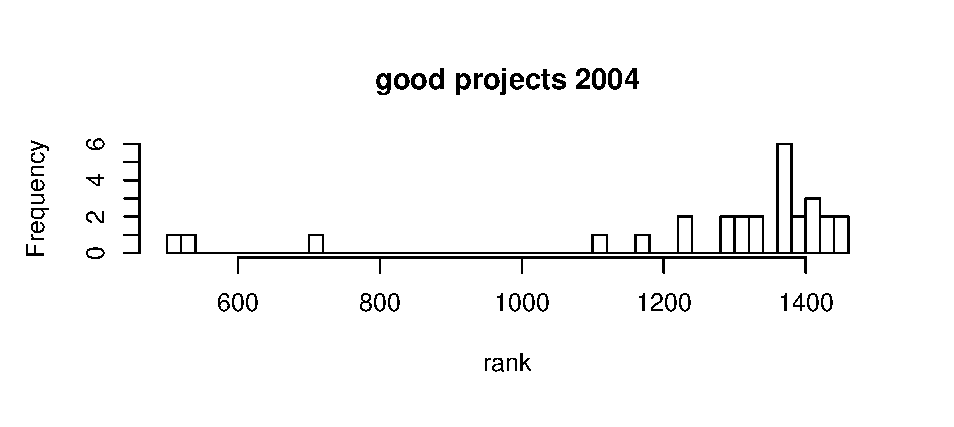
\includegraphics[width=0.3\textwidth]{figs/goodrank.eps}}	
	\subfloat[bad projects rank]{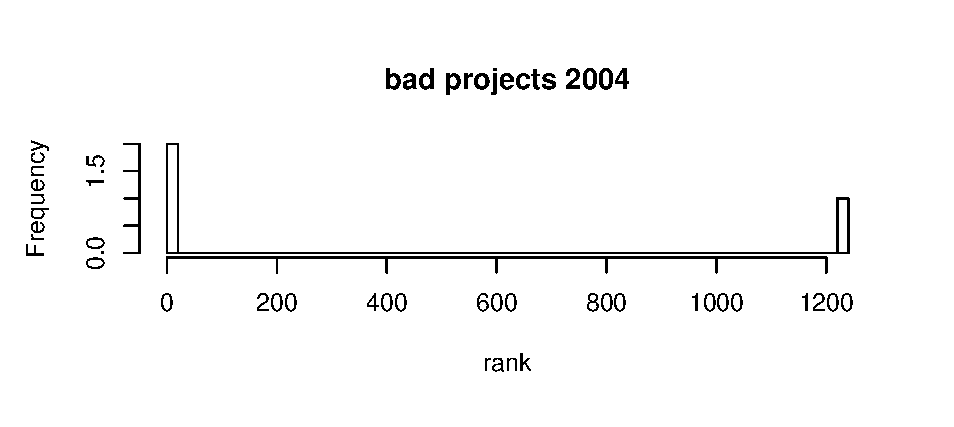
\includegraphics[width=0.3\textwidth]{figs/badrank.eps}}	
	\subfloat[moderate projects rank]{  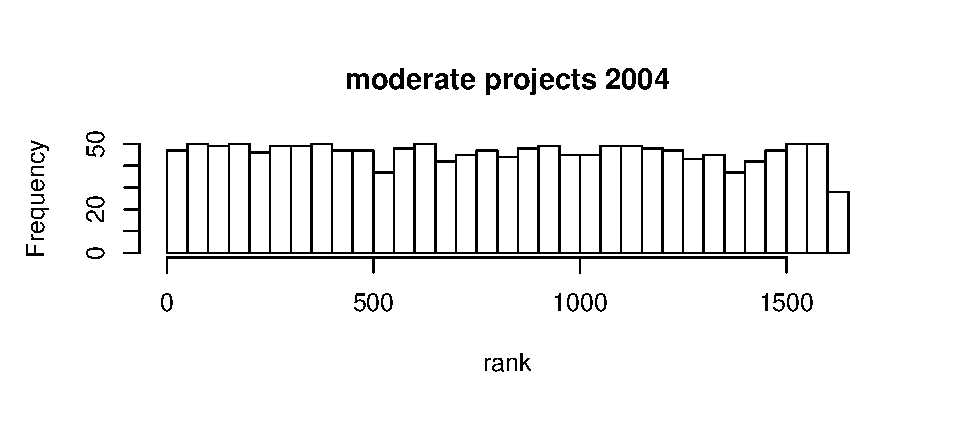
\includegraphics[width=0.3\textwidth]{figs/moderaterank.eps}}	
	\caption{original data without considering quantile}
\end{figure}



\begin{figure}
	\subfloat[Econ]{  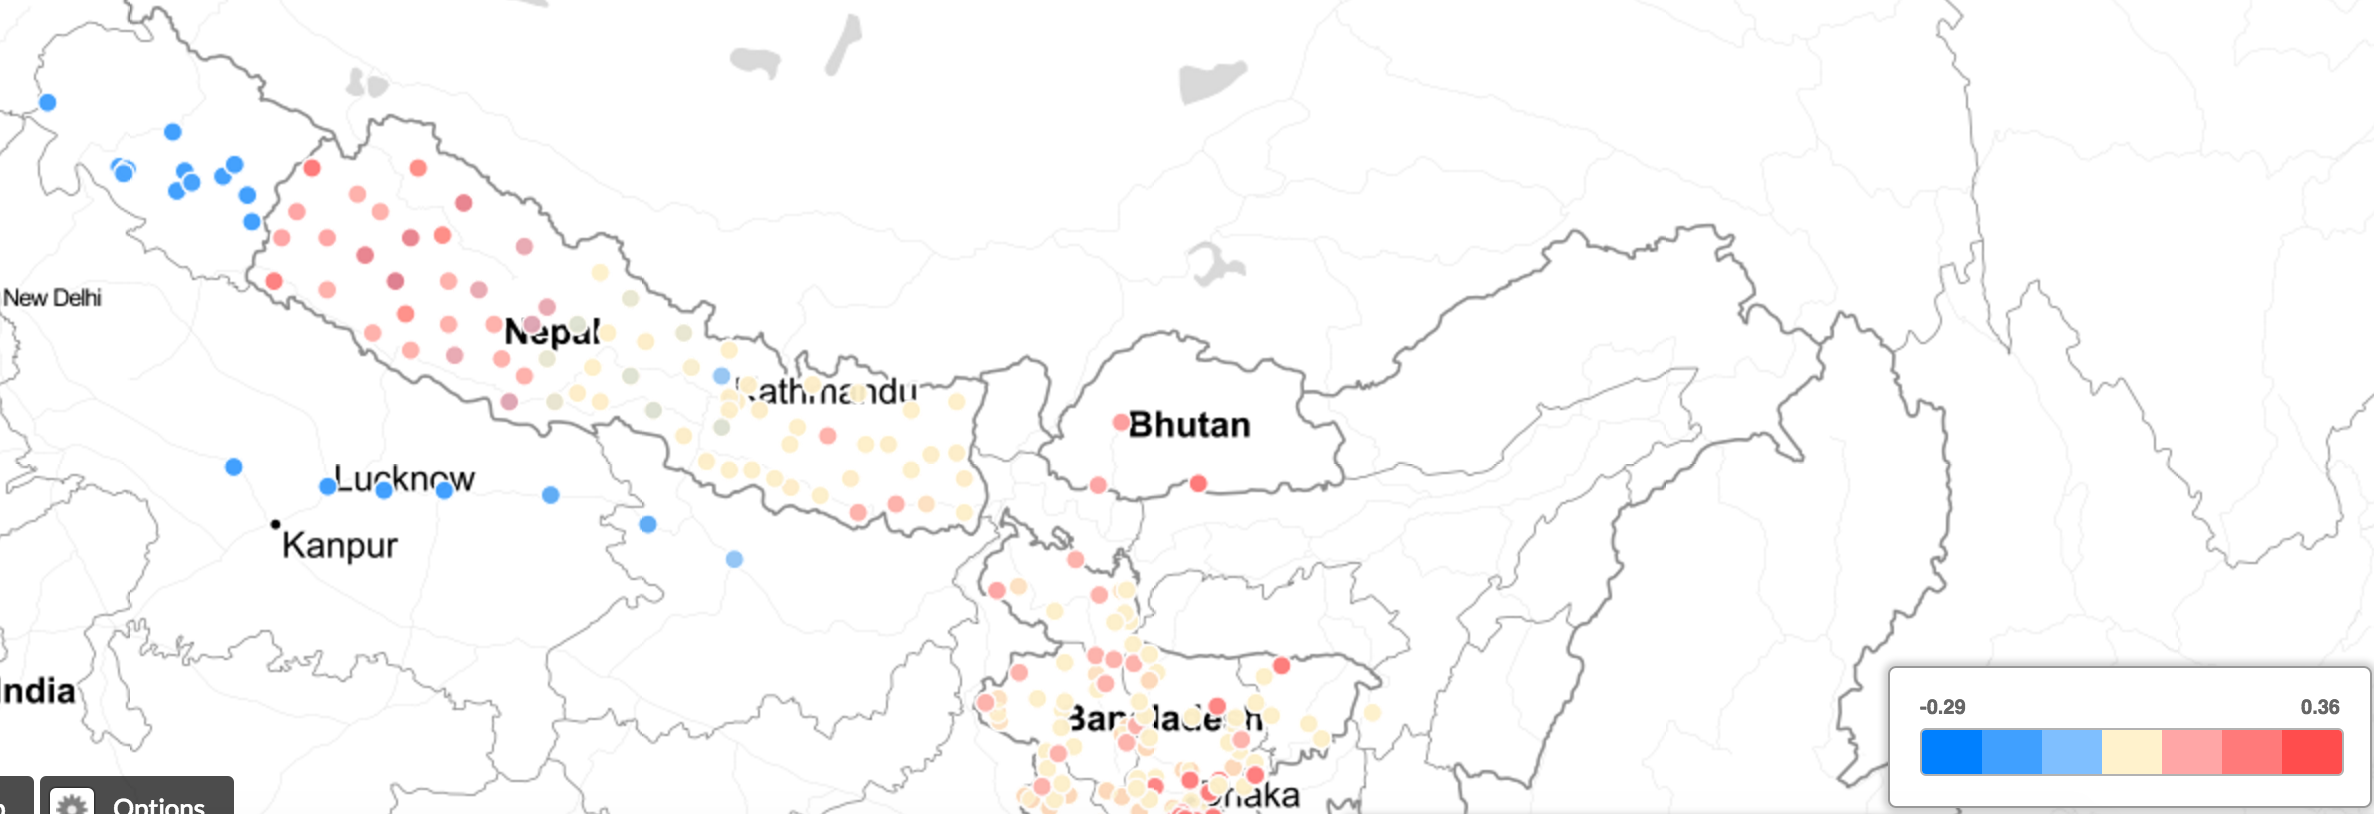
\includegraphics[width=0.35\textwidth]{figs/econmap.png}\label{fig:econ}}	
	\subfloat[Random Forest]{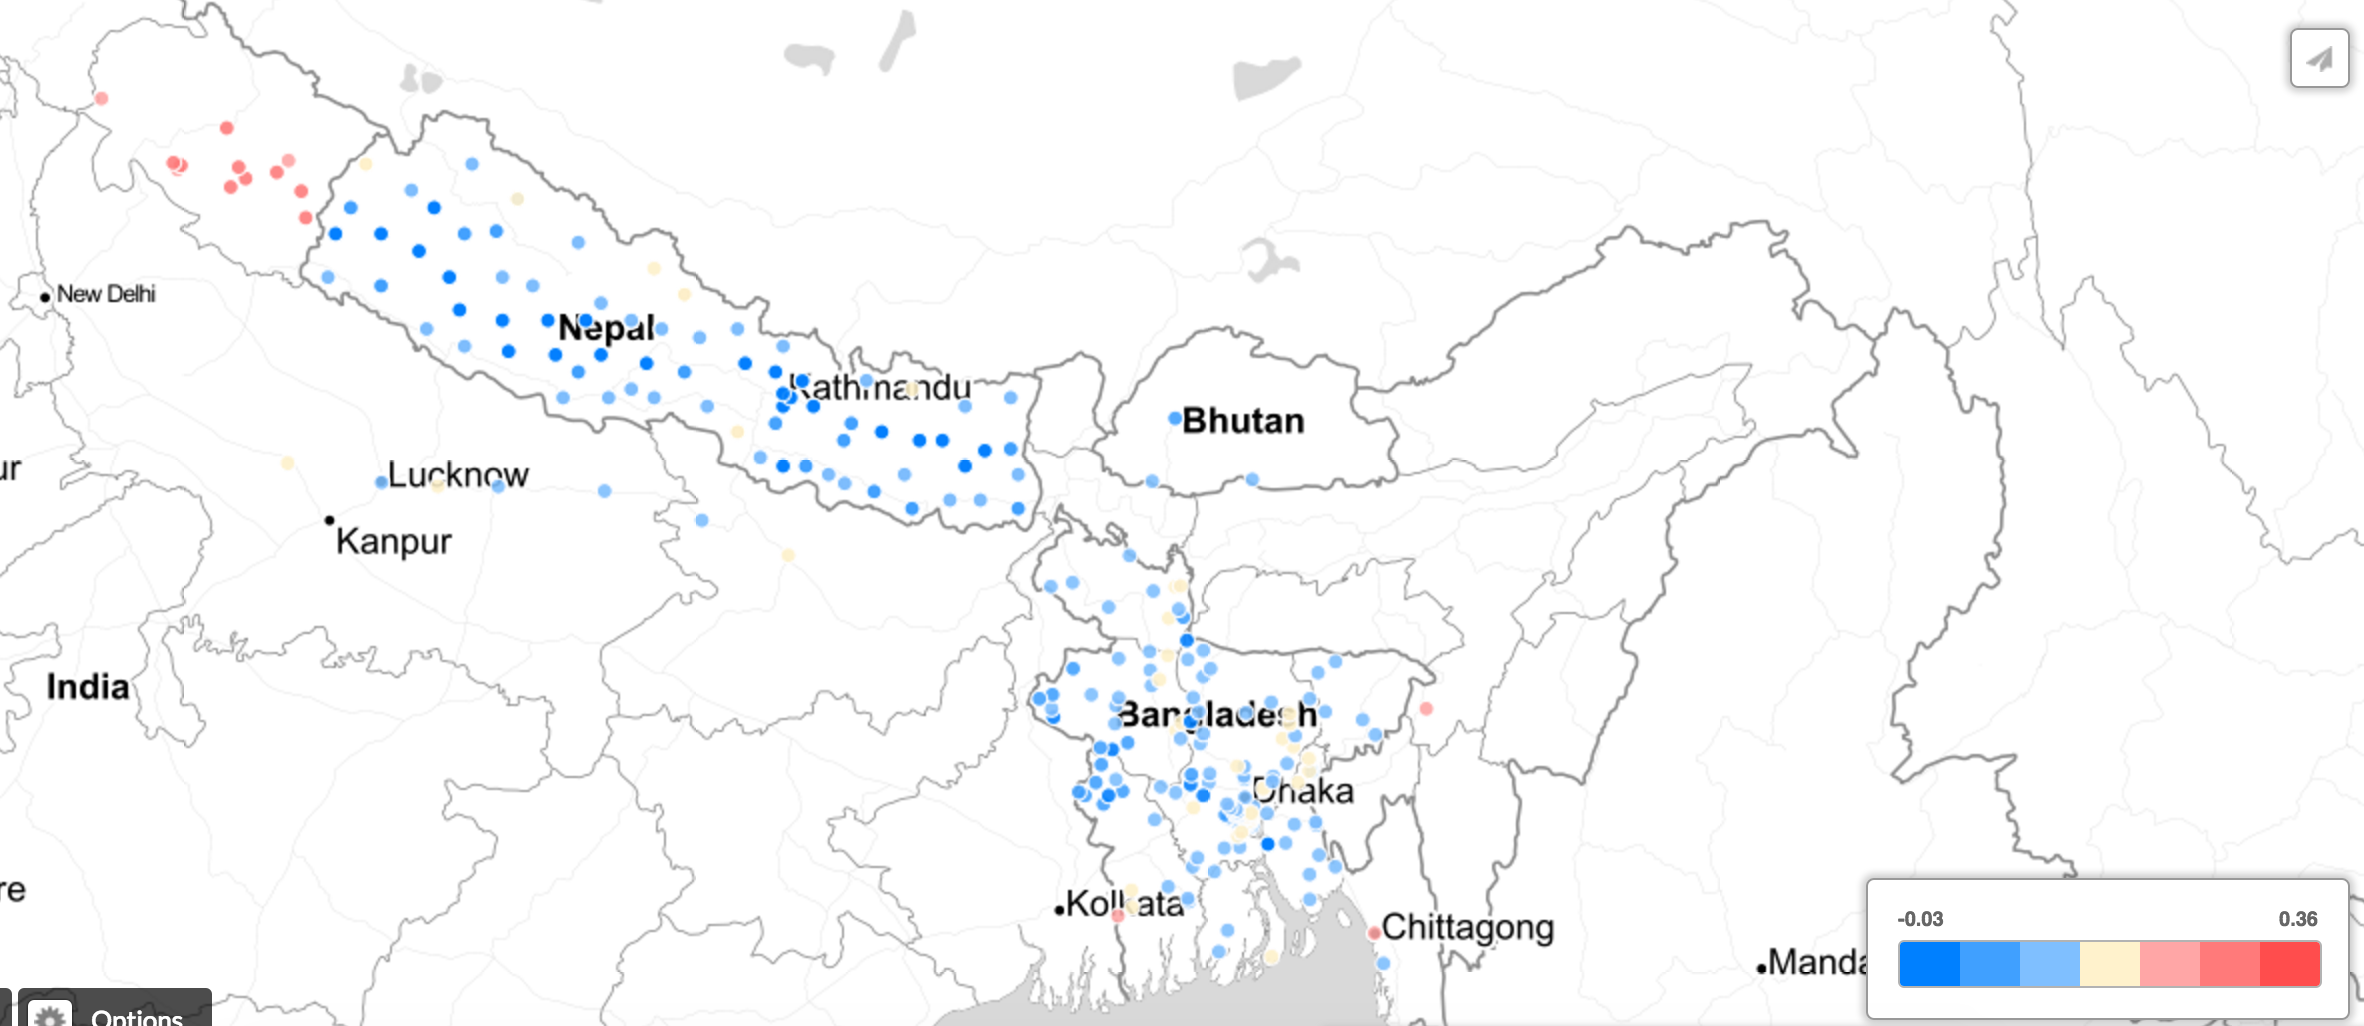
\includegraphics[width=0.35\textwidth]{figs/rfmap.png}\label{fig:rf}}	
	\subfloat[IEG outcome]{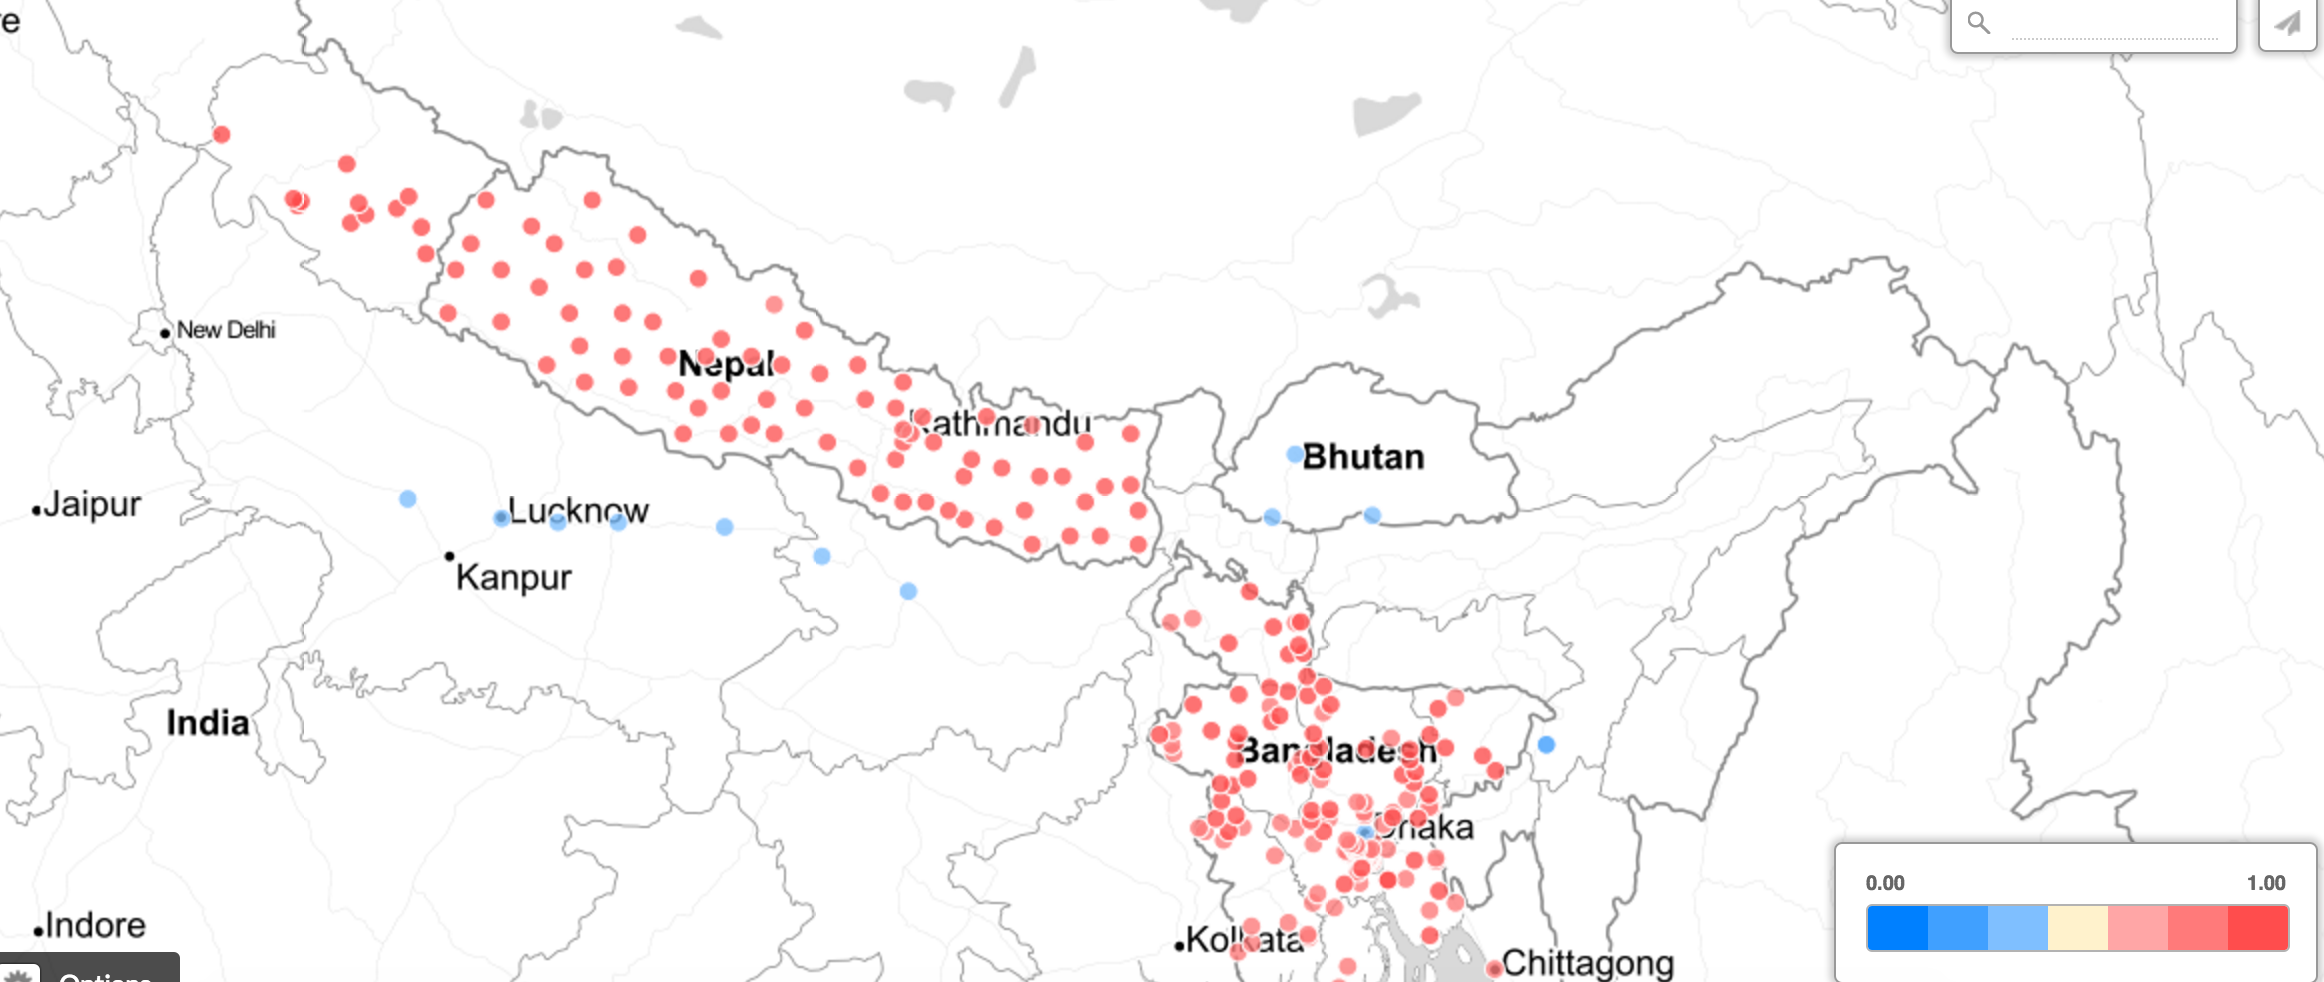
\includegraphics[width=0.35\textwidth]{figs/wbieg.png}\label{fig:ieg}}
	\caption{Nepal area 2004}
\end{figure}

\begin{figure}
	\subfloat[Econ]{  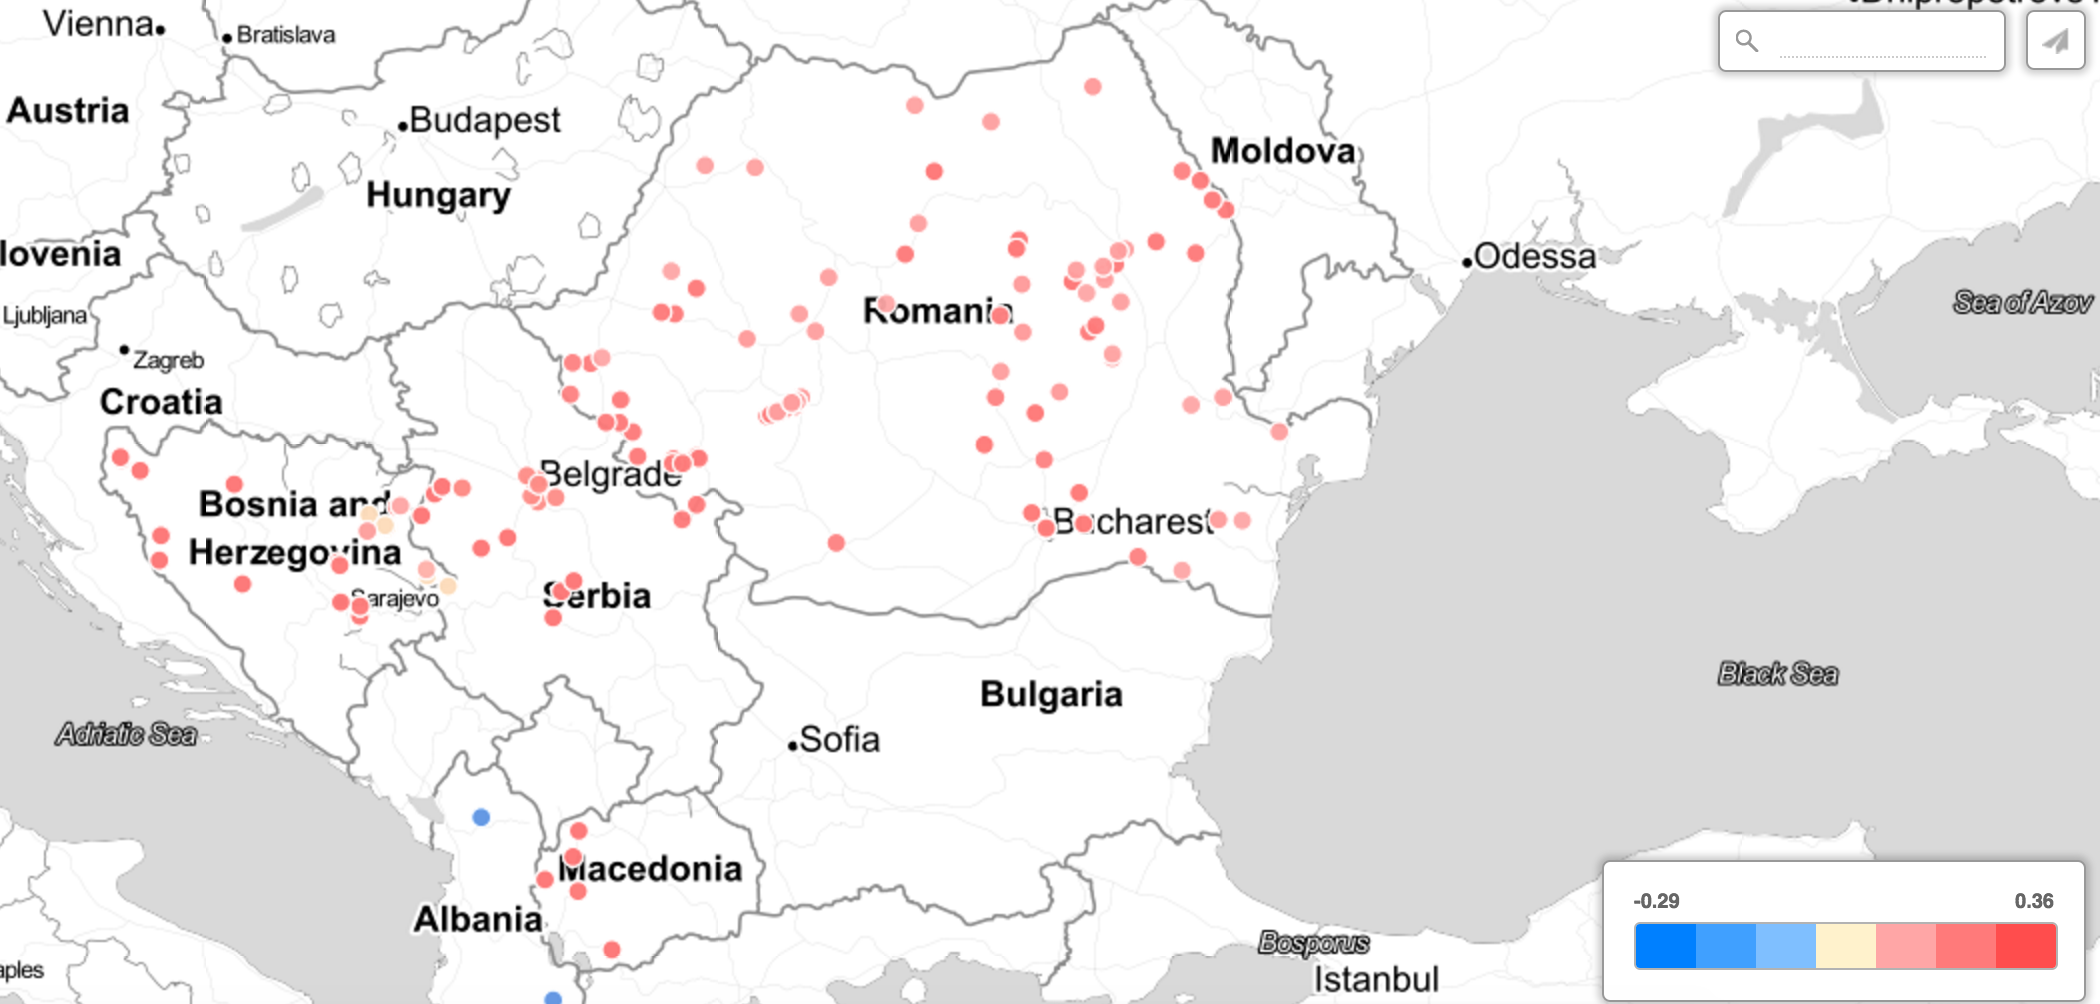
\includegraphics[width=0.35\textwidth]{figs/econeu.png}\label{figeu:econ}}	
	\subfloat[Random Forest]{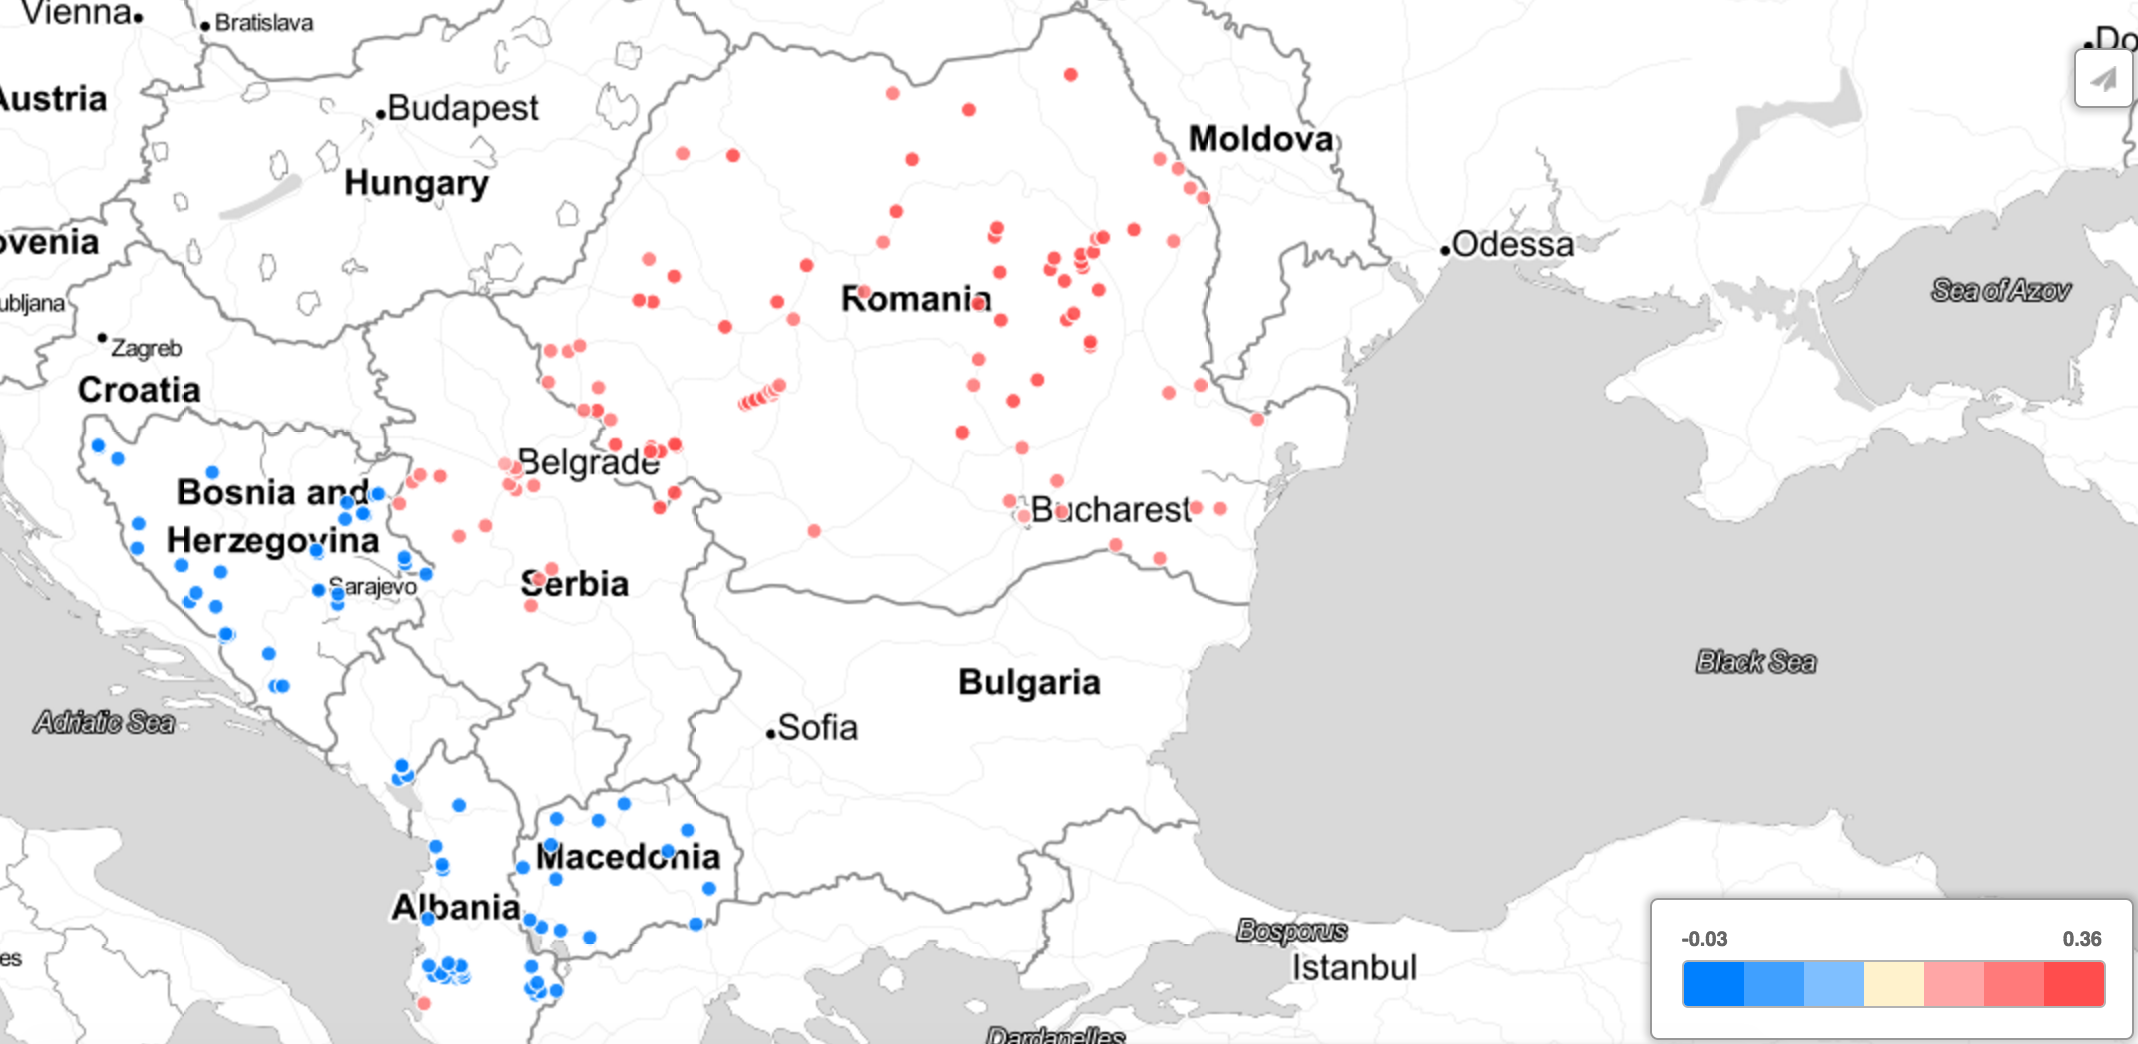
\includegraphics[width=0.35\textwidth]{figs/rfeu.png}\label{figeu:rf}}	
	\subfloat[IEG outcome]{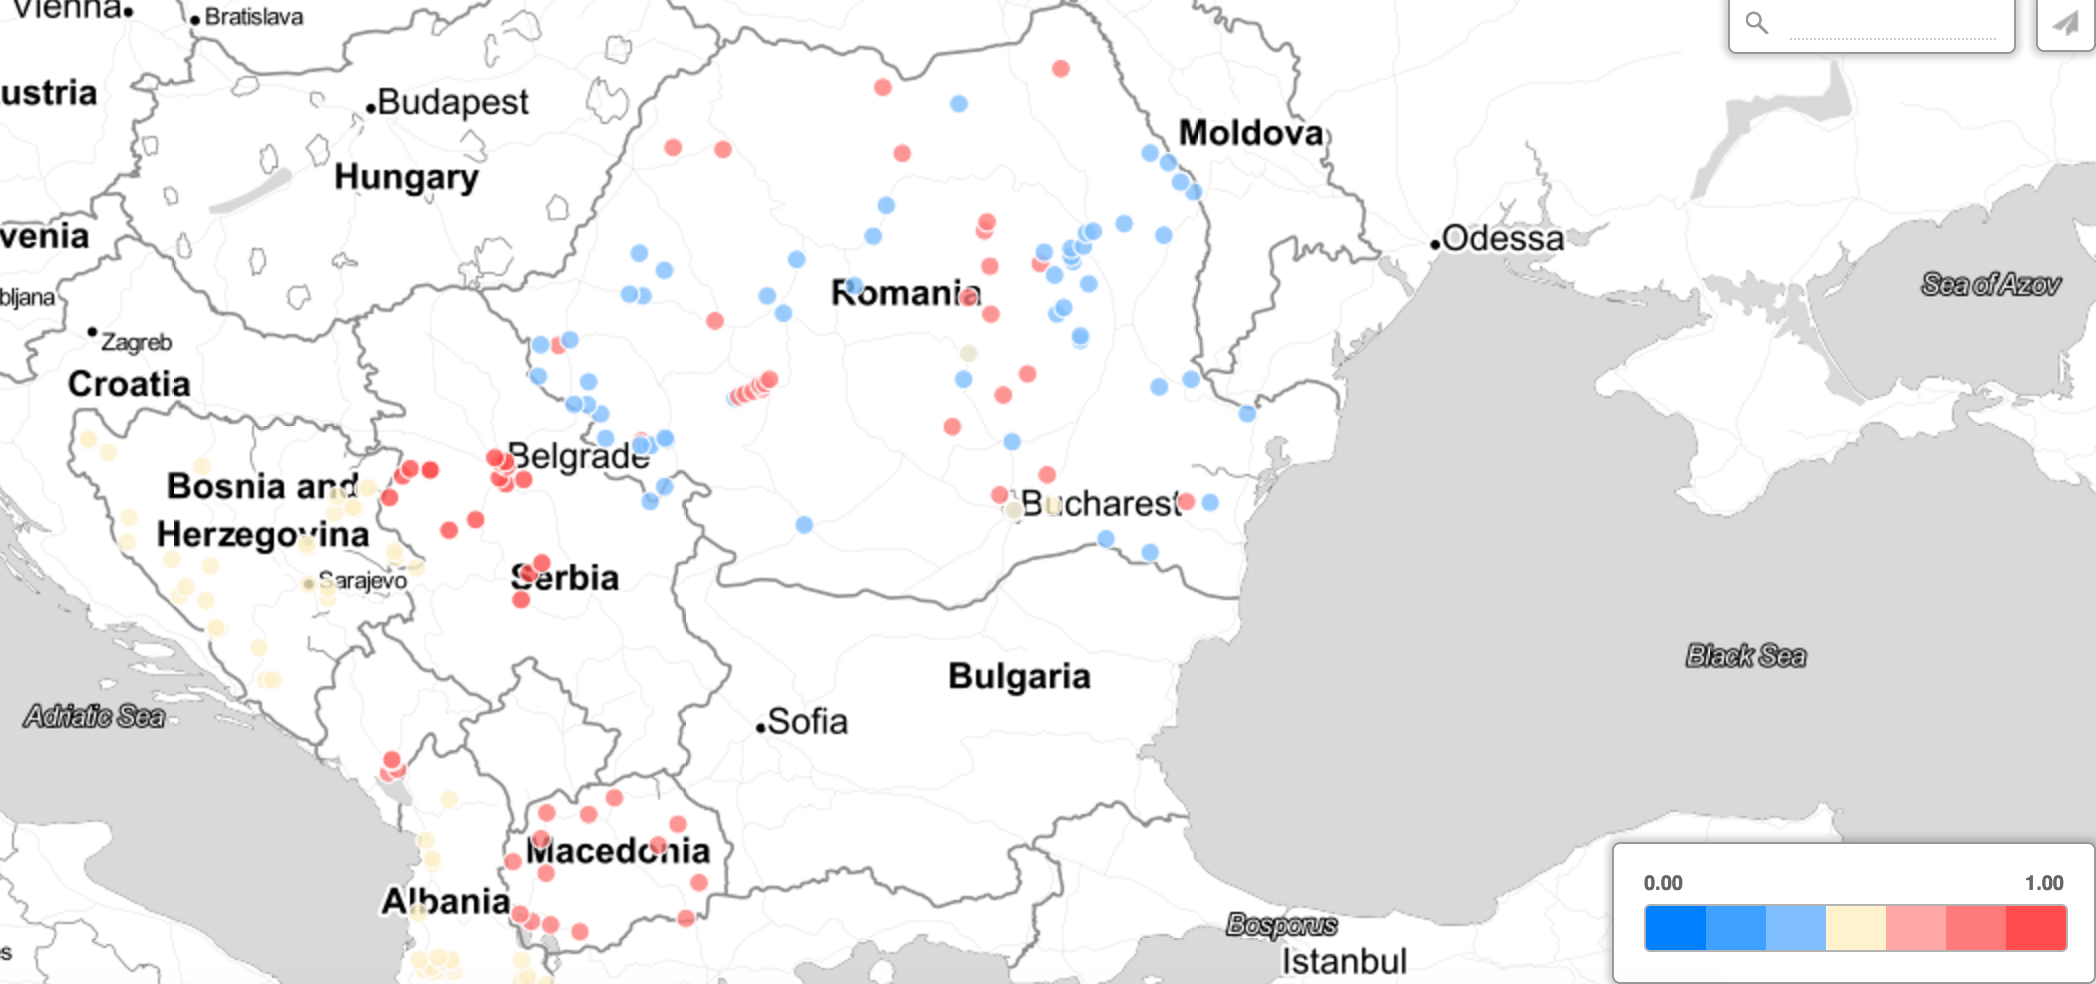
\includegraphics[width=0.35\textwidth]{figs/iegeu.png}\label{figeu:ieg}}
	\caption{East Europe}
\end{figure}



\begin{figure}
	\centering
	\subfloat[CT]{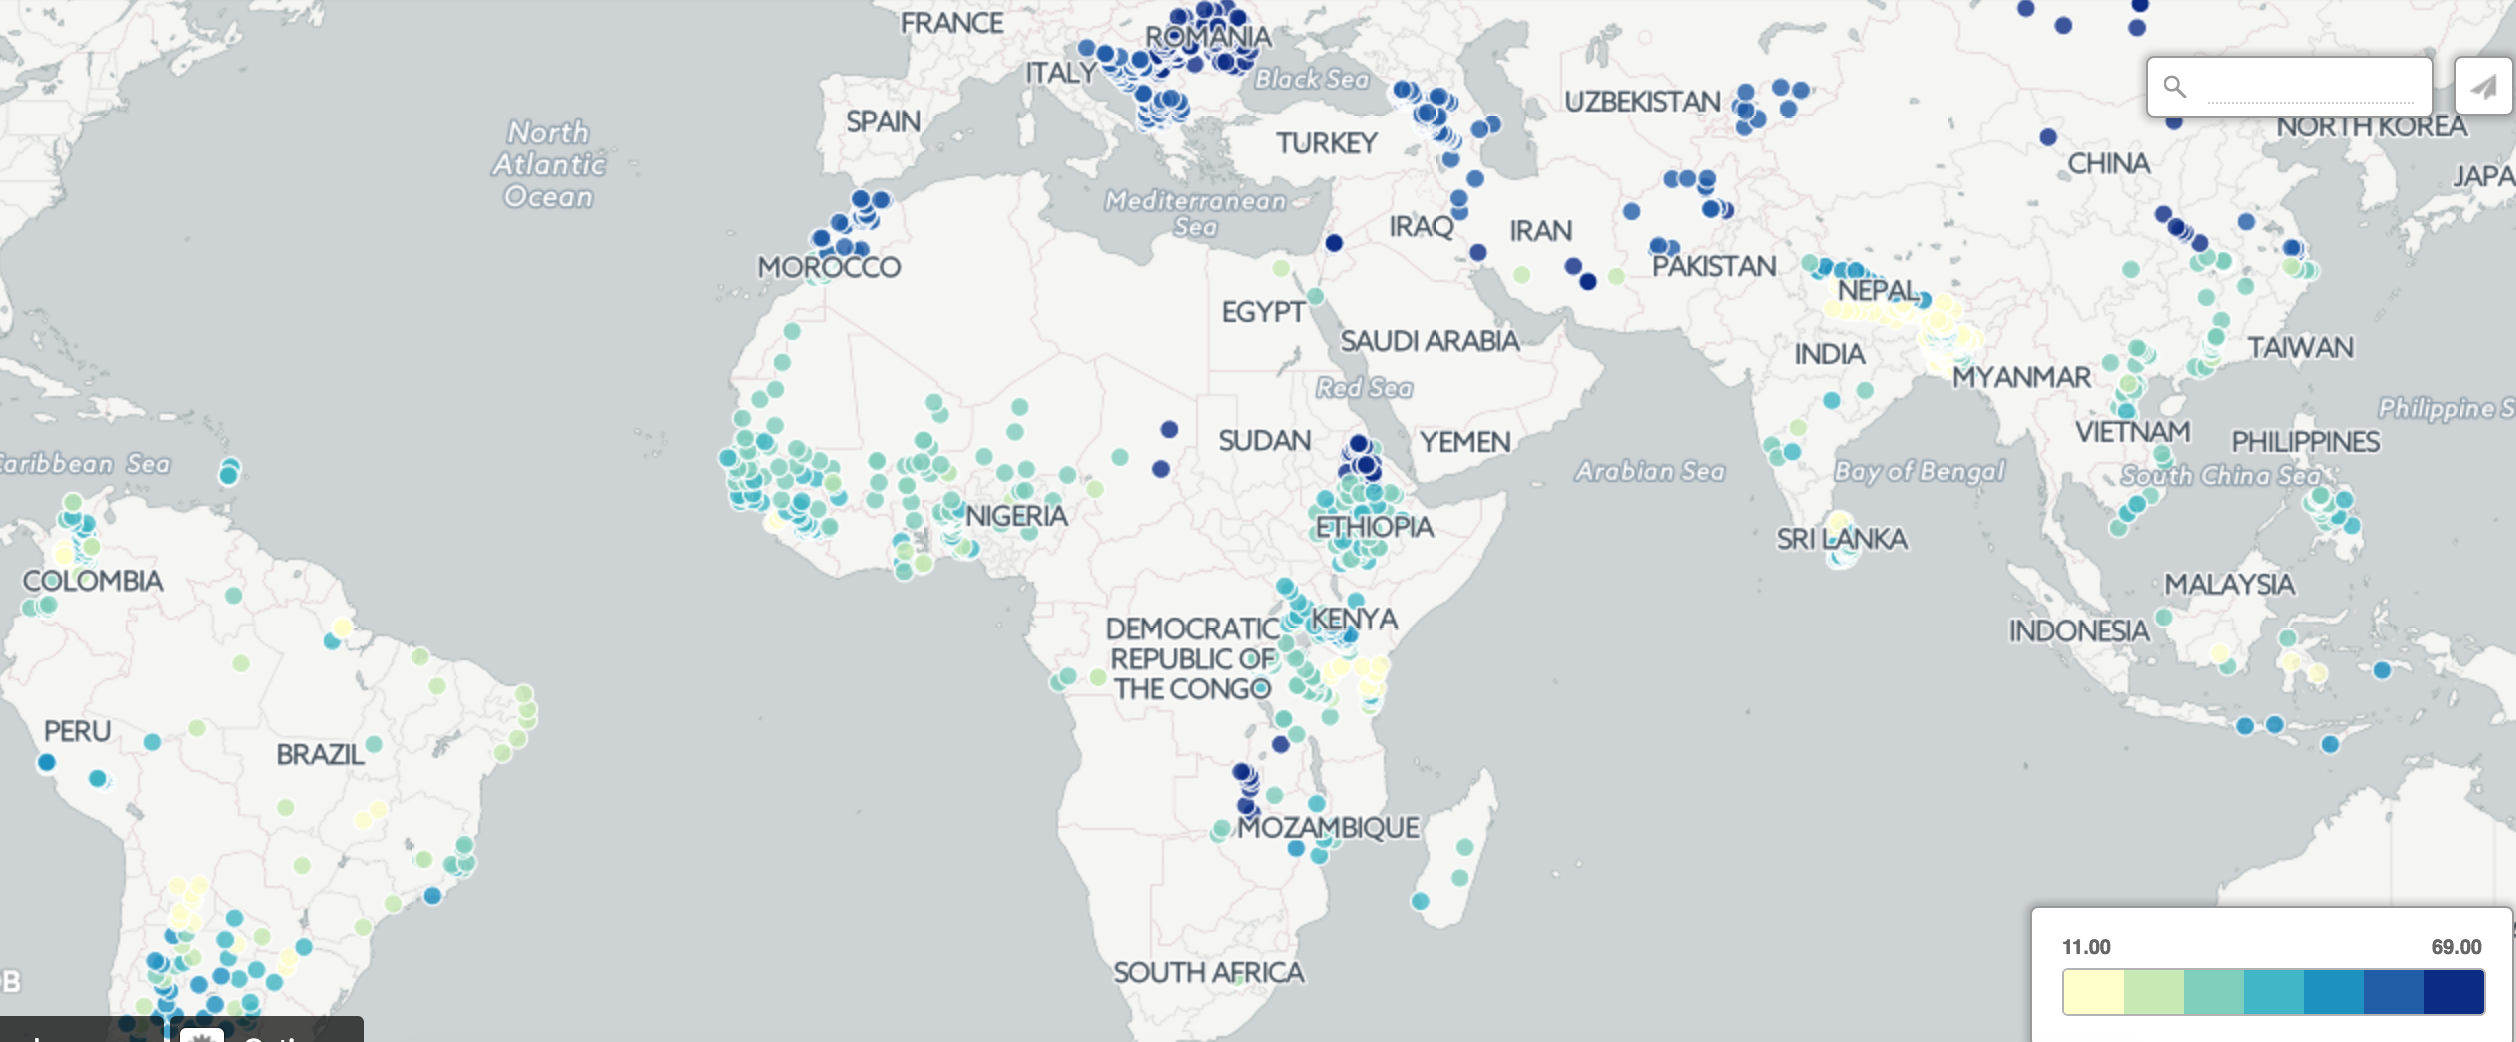
\includegraphics[width=0.5\textwidth]{figs/projectsbyleafct.png}}
	\subfloat[TOT]{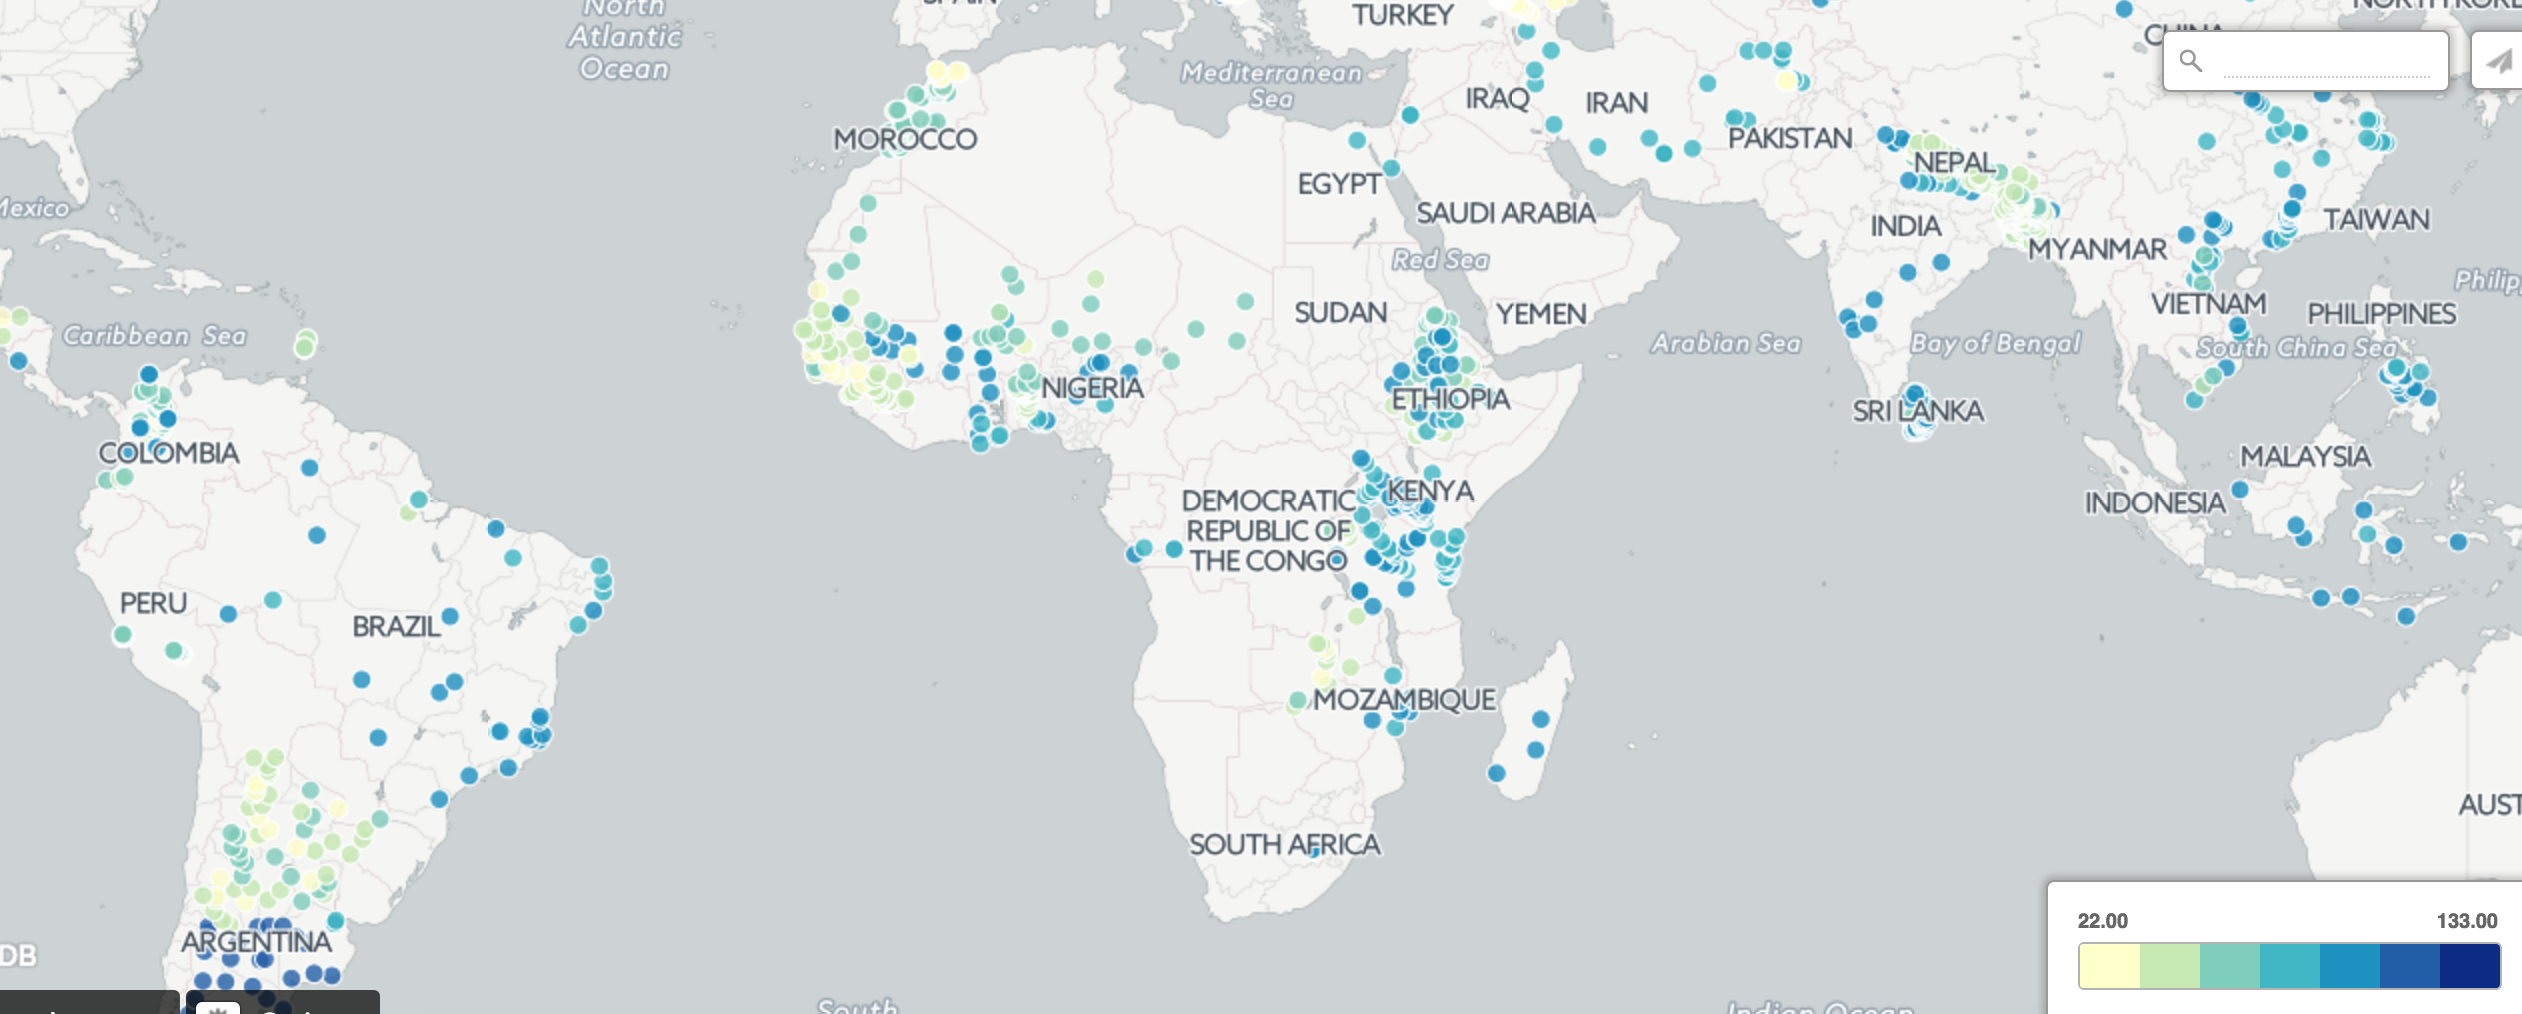
\includegraphics[width=0.5\textwidth]{figs/projectsbyleaftot.png}}
	\label{fig:leaf}
	\caption{projects colored by leaf they fall into }
\end{figure}


\begin{figure}
	\centering
	\subfloat[CT]{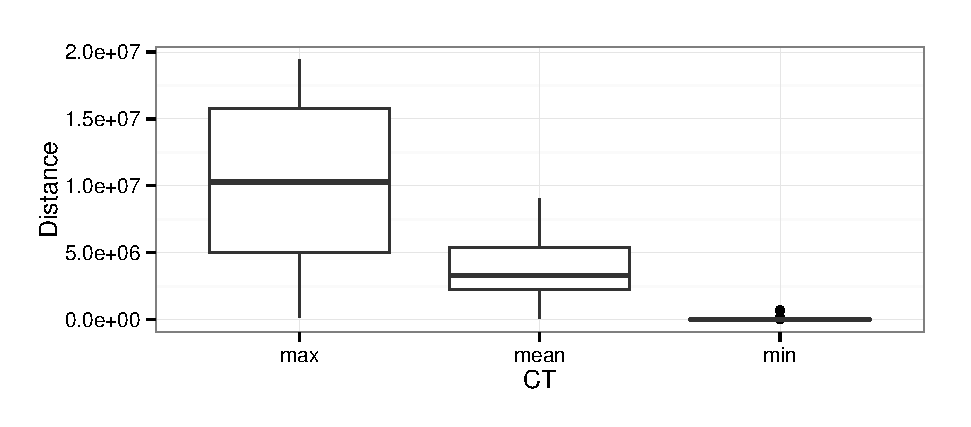
\includegraphics[width=0.5\textwidth]{figs/ctdist.eps}}
	\subfloat[TOT]{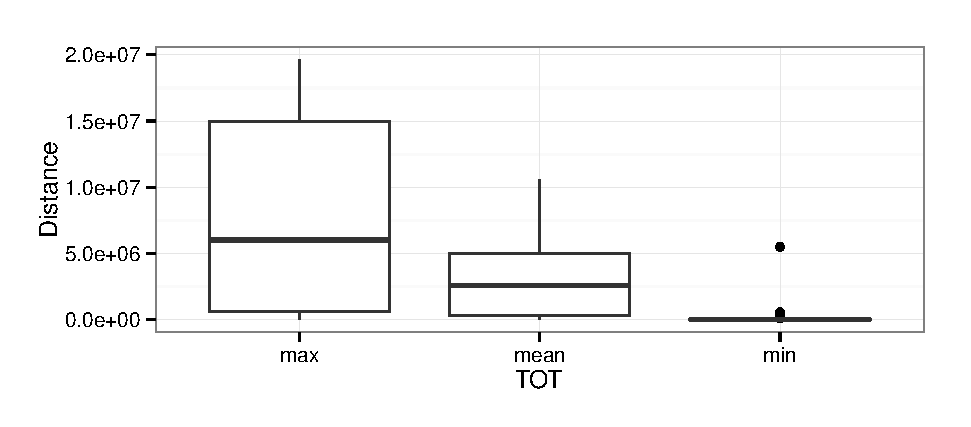
\includegraphics[width=0.5\textwidth]{figs/totdist.eps}}
	\label{fig:leafiest}
	\caption{distance within in the same leaf}
\end{figure}


\subsection{new data set}
Instead of the old data set with time series covariates, we establish the new data set which is the subset of the whole projects, which share the same project starting year, the starting years is between 2000 to 2012, project that started at 2000 has the largest number. We use projects start at 2000 to build the new data set.\\
In the new data set, we transform the time series covariate to the trend before the projects started and the trend after the project started along with the covariates with no time series. Then we use cross validation to choose the optimal complexity parameter and then use it to the new data set. 



\begin{figure}
	\centering
	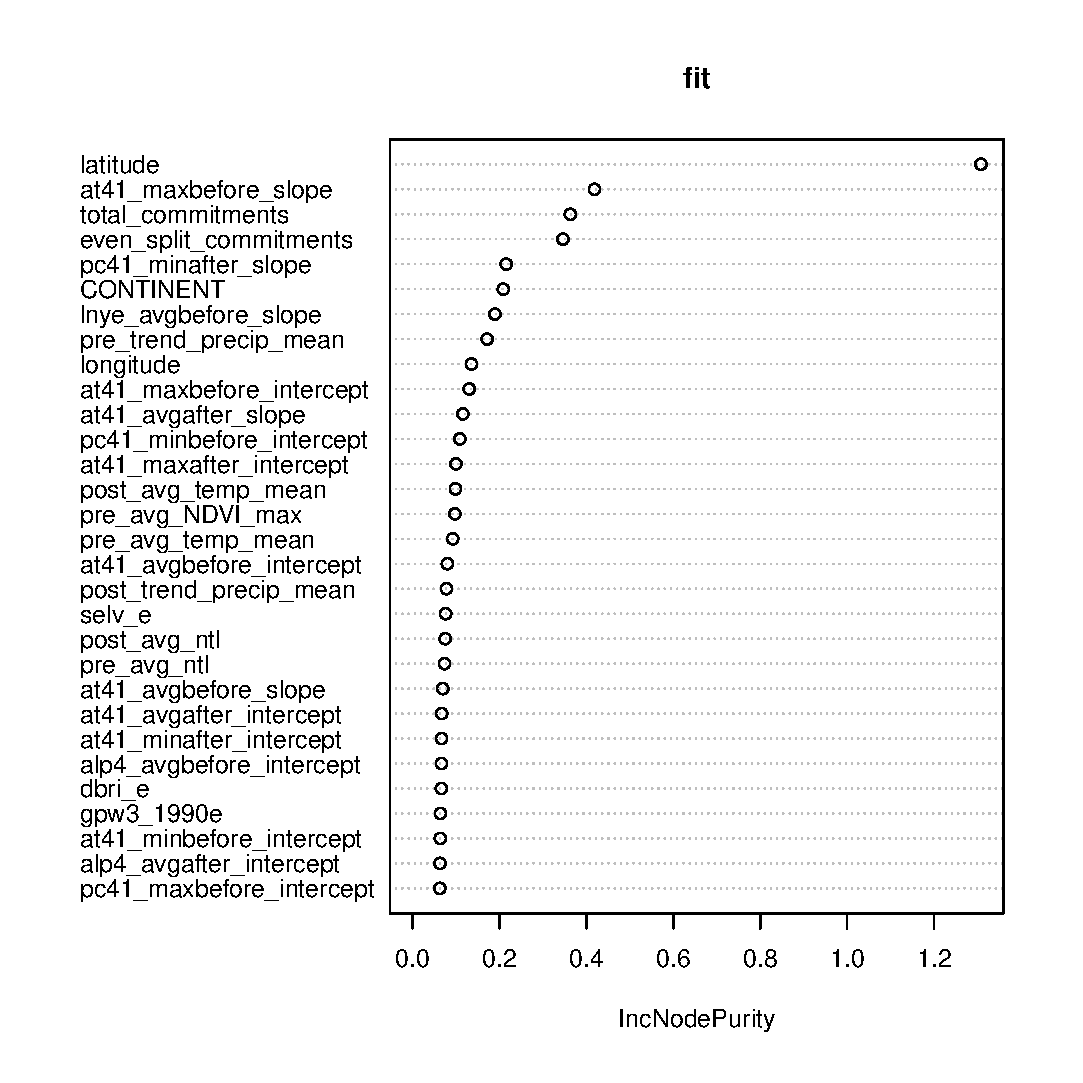
\includegraphics[width=0.6\textwidth]{figs/varimp2004.eps}
	\caption{variable importance 2004 projects}\label{fig:varimp}
\end{figure}

\begin{figure}
	\centering
	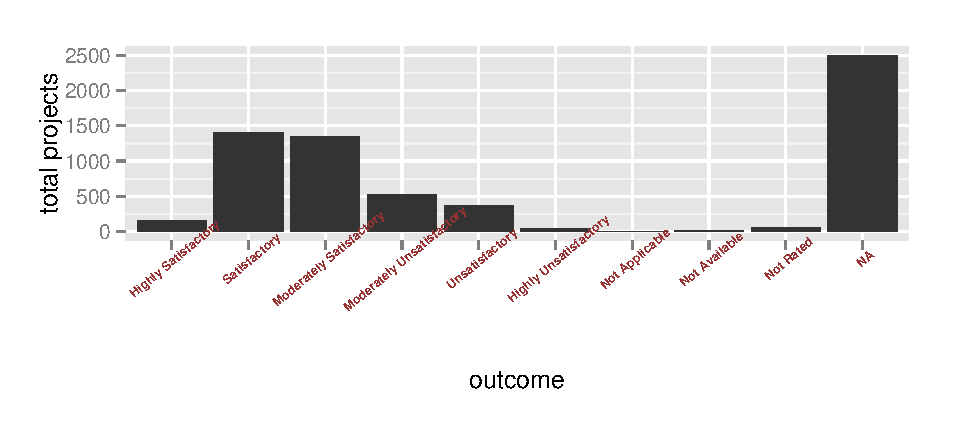
\includegraphics[width=\textwidth]{figs/hist_wb.eps}
	\caption{IEG outcome overview}
\end{figure}


 \begin{figure}
 \centering 
 \includegraphics[page=84,width=0.6\textwidth]{figs/project_2004.pdf}
 \caption{causal tree of projects in 2004}\label{fig:ct}
\end{figure}

\subsection{interpretation of results}
\begin{itemize}
\item Interpretation of data, what can we get out of the random forest?
From the random forest, we can observe the importance of each covariate as shown in \ref{fig:varimp} of year 2004. We can see that latitude is the most important among all the covariates, the other important factors includes the fund of the projects, the max temperature trend before the projects started. 
\item Anecdotal evidence, discuss best and worst project, what is it about, what happens here.

\item Numerical values for CATE? What is the exact interpretation of the calculated values (difficult thanks to propensity score weighting), but estimate of average should have a direct interpretation right? Interpret value for best and worst project.

\item Ranking of projects with respect to CATE?

\item Selection of variables / covariates are commonly selected among trees in the random forest? Provide details, interpret results. E.g. geographic location, show maps.

\item Comparison with an econometric model that looks at carbon foot print(?) Comparison with a world bank project evaluation from a human resources point of view.  In figure \ref{fig:ieg}, take the Nepal area for example, most of the projects are in the medium, neither good nor bad from the IEG outcome. In the random forest model, in figure \ref{fig:rf}, blue points are project in Nepal and the red points are projects in India, from this model, the cause effect in India is better that projects in Nepal, random forest model and economist model both have negative causal effect in Nepal, the difference between these two models is that projects have negative effect by economist model, but good effect by the random forest model. (what's the shortcoming of the econ model? ) In Nepal, the projects from the title are eduction and poverty alleviation projects, while in India they are Uttaranchal Decentralized Watershed project(how to explain?)Another example is the east Europe example, in both the random forest and economist model, they estimate Romain and Serbia projects achieve good effect while the effect is bigger in the random forest model than that in the economist model.In the IEG outcome, they evaluate the projects as moderate or unsatisfactory. The projects are Transport Restructuring Project, Mine Closure, Environment and Socio-Economic Regeneration Project, Modernizing Agricultural Knowledge and Information Systems Project (MAKIS).
In Bosnia and Herzegovina, random forest evaluate the projects has negative effect while the econ model rate them as positive, the projects title is Urban Infrastructure and Service Delivery Project. (No idea if these projects will cut trees or not or something else related with NDVI). The IEG outcome is Moderately Unsatisfactory for projects in this country. 


\item What do projects fall into the same leaf in the tree show in the map? In \ref{fig:leaf}, we can observe that both causal tree and transformed outcome tree would group projects nearby together, and we believe geographic information has big impact to the causal effect, which also in consistent with the important variable in the random forest. 

\end{itemize}
